\chapter{Dimensionality Reduction}
\section{Theory}
Dimensionality reduction is used to reduce the number of variables of the feature extraction.
There is two methods to make Dimensionality reduction, the first method is Fisher's linear discriminant model.
Fisher's model takes a D-dimensional input vector \textbf{x} and project to one dimension bye the equation:
\begin{equation}
y = \mathbf{w}^T \mathbf{x}.
\label{eq:fisher}
\end{equation} 

The projection down to one dimension leads to loss of information, and the data even if it was well separated in D-dimensions, can become overlapping when only viewed in one dimension.
The other method is Principal component analysis (PCA), which can be used to make a dimensionality reduction of the dataset.
PCA works bye orthogonal project the of the data onto a lower dimensional linear space.
The new space is called principal subspace and are made so that the variance of the projected data is maximized. 

\begin{figure}[H]
\centering
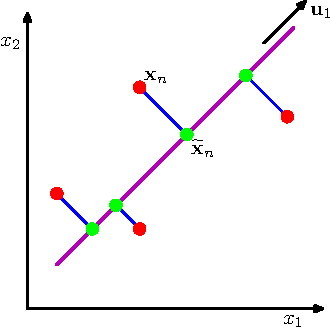
\includegraphics{Figure12_2_pdf}
\caption{Principal component analysis orthogonal project the of the data onto a lower dimensional linear space, This is shown on the figure. \fxnote{ref til bishop}}
\label{fig:dim_PCA_book}
\end{figure}

In this project PCA is used to make the dimensional reduction focusing on the maximum variance approach.

\subsection{Maximum Variance}
Consider a dataset of observations $ \left\lbrace \mathbf{x}_n \right\rbrace $ with $ n = 1,...,N $, and the data vector is a Euclidean variable with dimension D. 
The dataset can be projected to lower dimensional space with dimension $ M<D $ 	while maximizing the variance of the projected data. 
The projected space of dimension $ M $ is based on the eigenvectors $ \mathbf{u}_1, ..., \mathbf{u}_M $.
Consider a projection onto $ M=1 $ dimension, the projected space is spanned by the vector $ \mathbf{u}_1 $. 
Then each data point $ \mathbf{x}_n $ is projected onto a scalar $ \mathbf{u}_1^T \mathbf{x}_n $. The mean of the sample set is given by $ \overline{\mathbf{x}} \dfrac{1}{N}\sum_{n=1}^{N} \mathbf{x}_n $.
The calculate the variance of the projected data is given by
\begin{equation}
\dfrac{1}{N}\sum_{n=1}^{N}\left(\mathbf{u}_1^T \mathbf{x}_n-\mathbf{u}_1^T \overline{\mathbf{x}} \right)^2 = \mathbf{u}_1^T \mathbf{S} \mathbf{u}_1
\end{equation}
Where \textbf{S} is the covariance matrix. 
Then maximize the projected variance $ \mathbf{u}_1^T \mathbf{S} \mathbf{u}_1 $ with respect to $ \mathbf{u}_1 $.
Which show that the $ \mathbf{u}_1 $ is an eigenvector of \textbf{S}.
\begin{equation}
\mathbf{S}\mathbf{u}_1 = \lambda_1 \mathbf{u}_1
\end{equation}
Multiplying by $ \mathbf{u}_1 $ on the left.
\begin{equation}
\mathbf{u}_1^T \mathbf{S}\mathbf{u}_1 = \lambda_1
\end{equation}
The maximum of the variance is $ \mathbf{u}_1 $ is set equal to the eigenvector having the largest eigenvalue $ \lambda_1 $.
This eigenvector is called the first principal component. 
When $ M $ is set higher than 1, additional principal component can be defined by choosing each new direction that maximizes the projected variance.
This can be used to remove the dimensions that have small eigenvalue and therefore little information.         


\section{Method}
In this project PCA has been applied, mainly in an effort to improve the quality of the data by de-correlating it.
It has not been the focus to try and reduce the dimensionality of the data, as real-time processing cost has not been a deciding factor.
Subsequently, all analysis of classification methods has been done on data that has been de-correlated using PCA, but not reducing in dimensionality.

The effect og dimensionality reduction has though been studied, and is presented in this section

In order to gauge the effect of dimensionality of our data, we first analyse how much of the variance is contained in how many dimensions, and then look at the cost in accuracy of truncating dimensions of the de-correlated dataset.


\section{Results}

\subsection{Distribution of variance:}

\begin{figure}[H]
\centering
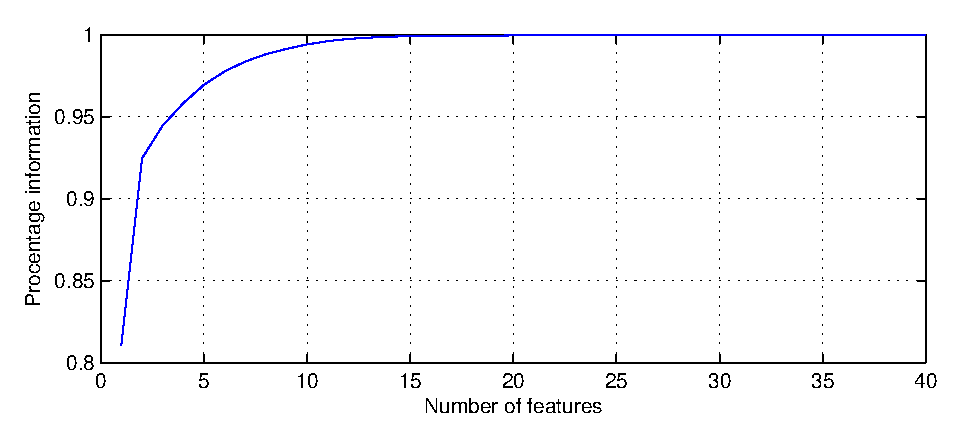
\includegraphics{PCA_dist_var}
\caption{Cumulative distribution of variance (information) in dimensions sorted by highest eigenvalue}
\label{fig:PCA_dist}
\end{figure}

\subsection{Cost of dimensionality reduction:}
The cost of dimensionality reduction is studied for linear classifiers and for Gaussian Mixture Models.

\subsubsection{Linear classifiers}

\begin{figure}[H]
\centering
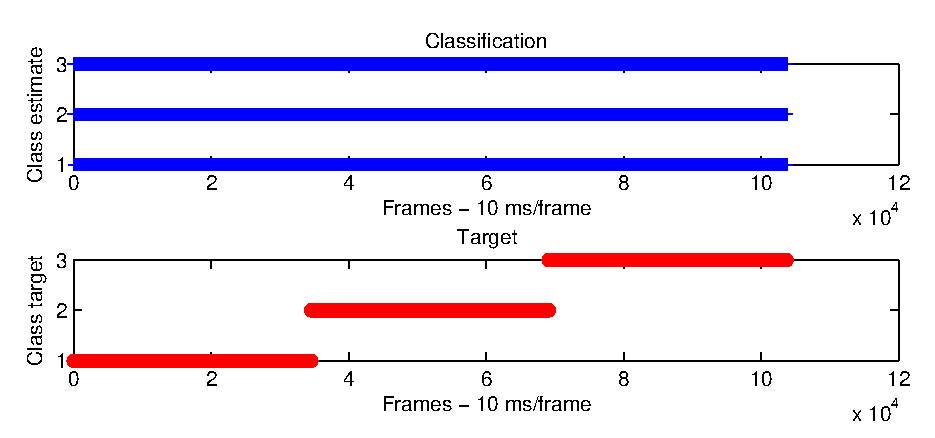
\includegraphics{Linear_10_PCA_trunc}
\caption{Results of using linear classifiers and ten digits spoken, with a truncated 10-dimensional feature space}
\label{fig:PCA_lin_trunc}
\end{figure}

\begin{table}[H]                                                           
\centering                                                                 
\begin{tabular}{|l|c|c|c|c|}                                               
\hline                                                                     
  & Speaker Jacob & Speaker Mose & Speaker Simon & Precision [\%] \\       
\hline                                                                     
Estimate Jacob & 16017.0 & 7631.0 & 6257.0 & 53.6 \\                       
\hline                                                                     
Estimate Mose & 9131.0 & 15367.0 & 7215.0 & 48.5 \\                        
\hline                                                                     
Estimate Simon & 9411.0 & 11561.0 & 21087.0 & 50.1 \\                      
\hline                                                                     
Sensitivity [\%] & 46.3 & 44.5 & 61.0 & 50.6 \\                            
\hline                                                                     
\end{tabular}                                                              
\caption{Confusion matrix - Linear classifier, truncated to 10 dimensions}
\label{table:Lin_conf_10_trunc}                                            
\end{table} 


\subsubsection{Gaussian Mixture Models}

\begin{figure}[H]
\centering
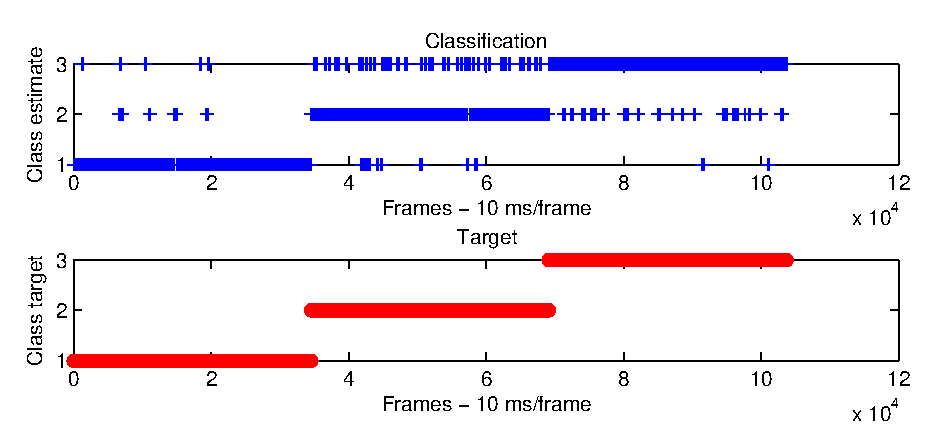
\includegraphics{GMM_10_PCA_trunc}
\caption{Results of using GMM and ten digits spoken, with a truncated 10-dimensional feature space}
\label{fig:PCA_GMM_trunc}
\end{figure}

\begin{table}[H]                                                    
\centering                                                          
\begin{tabular}{|l|c|c|c|c|}                                        
\hline                                                              
  & Speaker Jacob & Speaker Mose & Speaker Simon & Precision [\%] \\
\hline                                                              
Estimate Jacob & 33000.0 & 1400.0 & 300.0 & 95.1 \\                 
\hline                                                              
Estimate Mose & 959.0 & 27341.0 & 3200.0 & 86.8 \\                  
\hline                                                              
Estimate Simon & 600.0 & 5818.0 & 31059.0 & 82.9 \\                 
\hline                                                              
Sensitivity [\%] & 95.5 & 79.1 & 89.9 & 88.2 \\                     
\hline                                                              
\end{tabular}                                                       
\caption{Confusion matrix - GMM, truncated to 10 dimensions}        
\label{table:GMM_conf_10_trunc}                                     
\end{table} 



\section{Discussion}

Figure \ref{fig:PCA_dist} shows cumulative distribution of variance in the separate dimensions of the feature space.
In this it is apparent most of the variance is contained within the first 5-10 dimensions. 
$ 94.9 \% $ at 5 dimensions and $ 99.4 \% $ at 10 dimensions.
This does not necessarily imply that most of the information is contained within these, but is a good indicator of this.

The data shown in Figure \ref{fig:PCA_lin_trunc} and Table \ref{table:Lin_conf_10_trunc} for linear classifiers and Figure \ref{fig:PCA_GMM_trunc} and \ref{table:GMM_conf_10_trunc} for GMM, should be compared with Figure \ref{fig:Lin_fig_10} Table \ref{table:Lin_conf_10}, Figure \ref{fig:GMM_fig_10} and Table \ref{table:GMM_conf_10} respectively.

In this we see that truncating the feature space to one quarter of the dimensions (10) after PCA, has a very little effect on the overall accuracy of the classification.
This is important, since it can allow the classification algorithms to run with a much lower computational load.

In this project, computational load has not been a major concern. For this reason and the reason above it we have chosen not to truncate our feature space.